\documentclass[conference]{IEEEtran}
\IEEEoverridecommandlockouts

\usepackage{cite}
\usepackage{amsmath,amssymb}
\usepackage{algorithmic}
\usepackage{graphicx}
\usepackage{textcomp}
\usepackage{xcolor}
\usepackage{booktabs}
\usepackage{listings}
\usepackage{tikz}
\usetikzlibrary{arrows.meta,positioning,calc,fit,backgrounds}
\usepackage[hidelinks]{hyperref}

\lstset{
  basicstyle=\ttfamily\scriptsize,
  columns=fullflexible,
  keepspaces=true,
  breaklines=true,
  frame=none,
  aboveskip=4pt,
  belowskip=4pt,
}

\def\BibTeX{{\rm B\kern-.05em{\sc i\kern-.025em b}\kern-.08em
    T\kern-.1667em\lower.7ex\hbox{E}\kern-.125emX}}

% Semantic brackets, built from stock symbols so the paper needs no extra
% package beyond what IEEEtran already loads.
\providecommand{\llbracket}{\ensuremath{[\![}}
\providecommand{\rrbracket}{\ensuremath{]\!]}}

\begin{document}

\title{Proving Once, Applying Always: Offline Verified Rule Mining\\for
LLM-Assisted Compiler Optimisation}

\author{\IEEEauthorblockN{Darsh Sharma}
\IEEEauthorblockA{\textit{School of Computer Science and Engineering} \\
\textit{Vellore Institute of Technology}\\
Vellore, India \\
darsh.sharma2905@gmail.com}}

\maketitle

\begin{abstract}
Recent work on large language models for compiler optimisation has converged on
a single structural answer to the correctness problem: let the model generate
and let a formal checker decide. That answer is sound but it is paid for twice.
First, the checker runs out of road---Alive2 performs \emph{bounded}
translation validation over an intermediate representation that inherits C's
undefined behaviour, and a recent study reports roughly 20\% of a standard
vectorisation benchmark as unverifiable even after transformations intended to
make verification easier. Second, the model stays inside the build: reported
compile times reach 14 minutes per loop on benchmark kernels and 26 minutes on
real applications, and every compilation inherits the model's nondeterminism.
We describe ProveIt-C, a compiler that attacks both costs at once. We define
MiniC, a small imperative language whose semantics are \emph{designed} to be
verifiable: every operation either wraps or traps, nothing is undefined, and
peephole equivalence is therefore decidable in quantifier-free bitvector logic
rather than bounded. Proposals are expressed in a rule DSL whose operands and
constants are symbolic, so one solver query discharges every instance of a
pattern; proven rules are cached in a versioned library that the compiler
applies by pattern matching alone, with no inference in the build path. The
correctness obligation is \emph{trap-preserving} equivalence, which we show is
strictly stronger than value equivalence: a rewrite that masks a shift amount
to five bits agrees with the original on every input that produces a value and
is unsound only because it erases a trap. We report a partial implementation.
The front end, the verification core and the rule machinery are complete and
measured. We further report a first, small-scale measurement of the project's
headline question---how often a test-passing rewrite is nonetheless
wrong---using a live proposer (a single open-weight model served through a
third-party inference API, at temperature zero). Across 76 unscripted
proposals collected over three prompting iterations, the syntactically-invalid
rate fell from 84\% to 20\% to 3.8\% as we diagnosed and taught the model two
specific gaps between its assumptions and our rule grammar; three proposals
independently reproduced bug classes already present in our hand-written
adversarial corpus and were caught by the cheap differential-testing
prefilter; and of the 46 proposals that survived that prefilter, zero were
subsequently refuted by the solver at this sample size---a result we report
without generalising from, since the prompt used here favours well-known
textbook identities over risk-seeking optimisations, and a larger or more
adversarially-prompted sample may differ. Fourteen structurally distinct,
solver-proven, cost-reducing rules were accepted into the library from this
run; deduplicating them was itself necessary, since the model re-derived the
same identity under a different name in three separate, memoryless calls. On
a separate corpus of deliberately constructed near-miss rules built to
characterise the testing/proving gap directly, uniform random differential
testing plateaus at 73.3\% detection and does not improve across a
thousandfold increase in budget, boundary-seeded sampling reaches 93.3\% and
also plateaus, and one rule survives $7.8\times10^{6}$ trials across eight
tester configurations; the solver refutes all of them, in a median of
1.6\,ms. We also report two findings that were not anticipated: a rule
library admitted on soundness alone made every benchmark worse, because proof
and profitability are independent properties requiring separate machinery;
and the solver's verdict on queries containing two independent symbolic
multipliers is timing-dependent, which we handle by never allowing an
unsettled query to count as a proof.
\end{abstract}

\begin{IEEEkeywords}
compiler optimisation, translation validation, satisfiability modulo theories,
large language models, peephole optimisation, superoptimisation
\end{IEEEkeywords}

\section{Introduction}

A compiler does not get to be probably right. When a spreadsheet application
produces a wrong number the user usually sees it; when a compiler produces a
wrong instruction the program silently computes the wrong answer, and the fault
is attributed to the source code for as long as it takes someone to disbelieve
the compiler. This asymmetry is why compiler engineering treats a
miscompilation as categorically worse than a missed
optimisation~\cite{deadcode}, and why the
arrival of large language models in the optimisation pipeline is a correctness
question before it is a performance question. Models are fluent in proportion
to neither their correctness nor their own uncertainty~\cite{hallucination},
and an optimiser is a setting in which that mismatch is unusually expensive.

The field has answered that question in a consistent way. Taneja et
al.~\cite{llmvectorizer} observe that a transformation from LLVM IR to LLVM IR
can always be checked by Alive2~\cite{alive2} and the original returned on
failure, so that the model need not be trusted at all. Fang et
al.~\cite{llmveriopt} take the same observation into training, using Alive2's
verdict as a reward signal for reinforcement learning. Kwon et
al.~\cite{cov} accept the observation and extend it with a runtime layer for
the cases the checker cannot settle. The common shape---generate freely,
verify deterministically, fall back on failure---is now well established, and
we adopt it without claiming it.

What we claim concerns the two costs that shape leaves in place.

\textbf{The checker runs out of road.} Alive2 is, by its own title, a
\emph{bounded} translation validator. The boundedness is not an implementation
shortcoming; it follows from the object being checked. LLVM IR~\cite{llvm}
inherits C's undefined behaviour, and modelling it faithfully requires
\texttt{poison} and \texttt{undef} together with a memory model whose SMT
encoding is a research contribution in its own right~\cite{smtmemory}. The consequences are visible in
the measurements. Kwon et al. report that approximately 20\% of the TSVC
loops~\cite{tsvc} they study resist verification even after LLM-Vectorizer has
applied unrolling, alias annotations and alignment enforcement specifically to
make them verifiable~\cite{cov}; they conclude that a runtime mechanism is
required, and build one. Fang et al. simply exclude timeouts and
undefined-behaviour-triggering pairs from their training set~\cite{llmveriopt},
and note in their discussion that Alive2 returns wrong answers on a small
number of loop-carrying test cases.

\textbf{The model stays in the build.} In every system cited above, compiling a
program means running a language model. LLM-VeriOpt invokes a 3B-parameter
model per function; CoV invokes a 671B-parameter model and reports an average
compile time of about 14 minutes per loop on TSVC and 26 minutes on real
applications, dominated by inference and solver calls~\cite{cov}. Beyond the
wall-clock cost, this makes the build itself nondeterministic in a way
engineers have spent two decades removing: reproducible builds, bit-identical
artefacts and cacheable compilation all assume the compiler is a function of
its inputs.

\subsection{Approach}

ProveIt-C attacks these costs from two directions that reinforce each other.

\textit{Define the undefined behaviour away rather than model it.} We introduce
MiniC, a small imperative language in which signed arithmetic wraps, division
by zero traps, an out-of-range shift traps, and an out-of-bounds array access
traps. There is no undefined behaviour, so there is no need for \texttt{poison}
or \texttt{undef}, and equivalence of loop-free fragments is decidable in
QF\_BV. A proof is total rather than bounded. The price is scope, and we state
it throughout: MiniC is not C, and no measurement here is a measurement about
C.

\textit{Prove generalised rules offline so the build needs no model.} A
proposal is not a rewritten function but a \emph{rule} in a small DSL modelled
on Alive's~\cite{alive}, in which operands and constants are symbolic. A single
\texttt{unsat} therefore covers every instance of the pattern rather than the
one instance the proposer examined. Proven rules accumulate in a versioned
library, and the compiler consults that library by pattern matching. Mining is
expensive, offline and eventually model-driven; compilation is a pattern match.
The model's nondeterminism is spent once, at mining time, instead of on every
build.

Fig.~\ref{fig:arch} shows the resulting split. The upper band runs once per
rule, is expensive, and is where a model belongs; the lower band runs on every
compilation and contains no inference at all. The rule library is the only
channel between them, and it carries proofs rather than predictions.

A third element emerges from the first. Because traps are observable in MiniC,
the obligation the solver discharges is \emph{trap-preserving} equivalence:
both sides must trap on exactly the same inputs and agree on values everywhere
else. This is strictly stronger than value equivalence, and the difference is
not academic. Our adversarial corpus contains a rewrite that masks a shift
amount to five bits---precisely what x86 and ARM hardware does. It agrees with
the original on every input that yields a value. It is unsound, and our checker
refutes it, only because the original traps on a shift of 32 and the rewrite
does not. A checker that compared values alone would admit it.

\begin{figure*}[!t]
\centering
% The drawing is a few points wider than \textwidth; scaling it to fit is
% uniform and imperceptible, and keeps the figure inside the column measure.
\resizebox{\textwidth}{!}{%
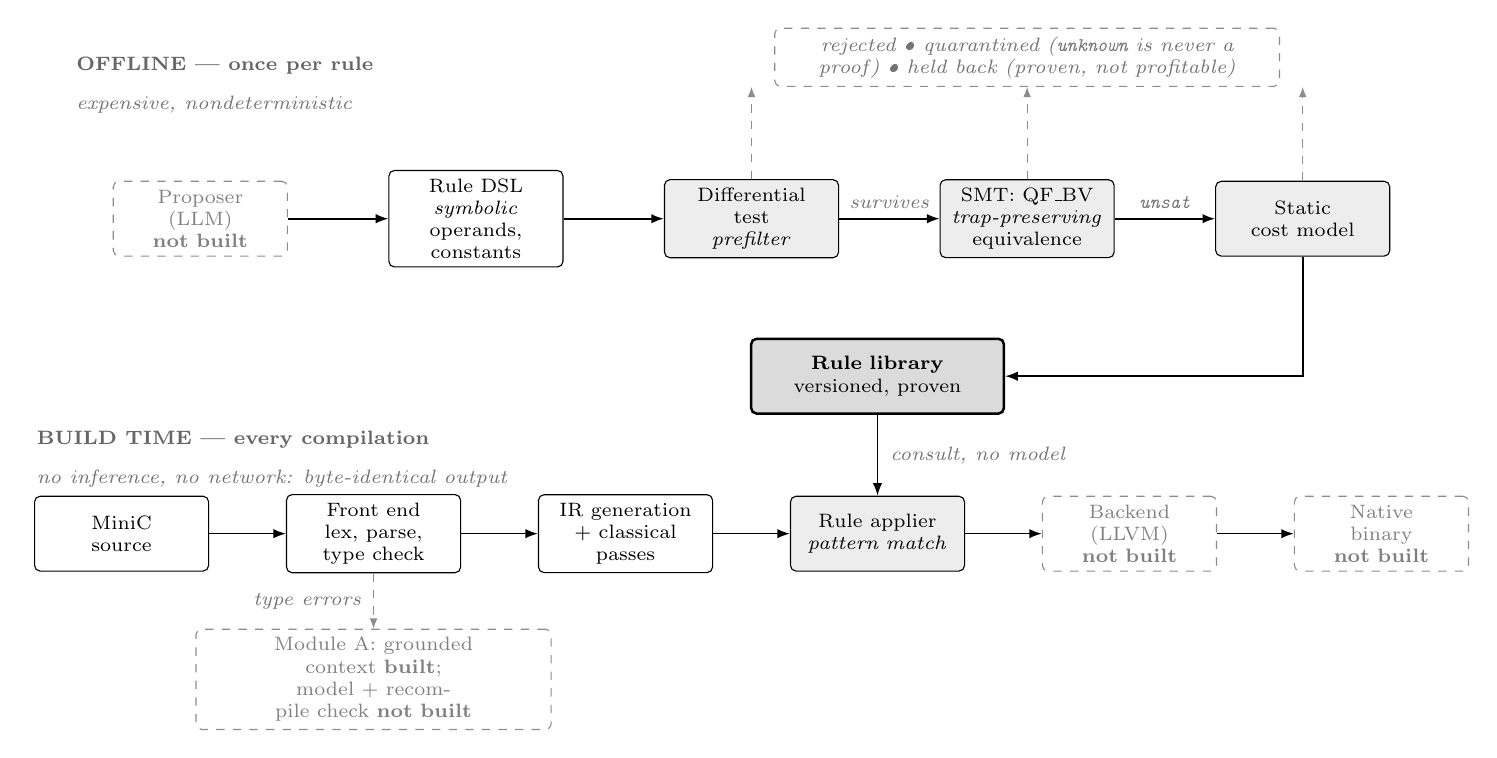
\begin{tikzpicture}[
  font=\scriptsize,
  stage/.style   ={draw, rounded corners=2pt, align=center, inner sep=3pt,
                   minimum height=9.5mm, text width=20mm},
  gate/.style    ={stage, fill=black!7},
  store/.style   ={stage, fill=black!14, line width=0.9pt, text width=30mm},
  future/.style  ={stage, dashed, draw=black!45, text=black!50},
  sink/.style    ={draw=black!45, dashed, rounded corners=2pt, align=center,
                   inner sep=3pt, text width=62mm, font=\scriptsize\itshape,
                   text=black!55},
  band/.style    ={font=\scriptsize\bfseries, text=black!60, anchor=west},
  note/.style    ={font=\scriptsize\itshape, text=black!55},
  ar/.style      ={-{Latex[length=1.6mm]}, semithick},
  rj/.style      ={-{Latex[length=1.3mm]}, draw=black!45, dashed},
]

% ---------------- offline band: once per rule, model in the loop ----------
\node[band] at (-8.7, 3.95) {OFFLINE\ \textemdash\ once per rule};
\node[note] at (-8.7, 3.45) [anchor=west] {expensive, nondeterministic};

\node[future] (prop)  at (-7.0, 2.0) {Proposer\\(LLM)\\\textbf{not built}};
\node[stage]  (dsl)   at (-3.5, 2.0) {Rule DSL\\\emph{symbolic}\\operands, constants};
\node[gate]   (dt)    at ( 0.0, 2.0) {Differential\\test\\\emph{prefilter}};
\node[gate]   (smt)   at ( 3.5, 2.0) {SMT: QF\_BV\\\emph{trap-preserving}\\equivalence};
\node[gate]   (cost)  at ( 7.0, 2.0) {Static\\cost model};

\draw[ar] (prop) -- (dsl);
\draw[ar] (dsl)  -- (dt);
\draw[ar] (dt)   -- node[above,note]{survives} (smt);
\draw[ar] (smt)  -- node[above,note]{\texttt{unsat}} (cost);

% ---------------- what each gate throws away ------------------------------
\node[sink] (rej) at (3.5, 4.05)
  {rejected \textbullet\ quarantined (\texttt{unknown} is never a proof)
   \textbullet\ held back (proven, not profitable)};
\draw[rj] (dt.north)   -- (rej.south -| dt.north);
\draw[rj] (smt.north)  -- (rej.south -| smt.north);
\draw[rj] (cost.north) -- (rej.south -| cost.north);

% ---------------- the only channel between the two bands ------------------
\node[store] (lib) at (1.6, 0.0) {\textbf{Rule library}\\versioned, proven};
\draw[ar] (cost.south) |- (lib.east);

% ---------------- build band: every compilation, no model -----------------
\node[band] at (-9.2, -0.80) {BUILD TIME\ \textemdash\ every compilation};
\node[note] at (-9.2, -1.30) [anchor=west]
  {no inference, no network: byte-identical output};

\node[stage]  (src)  at (-8.0, -2.0) {MiniC\\source};
\node[stage]  (fe)   at (-4.8, -2.0) {Front end\\lex, parse,\\type check};
\node[stage]  (irg)  at (-1.6, -2.0) {IR generation\\+ classical\\passes};
\node[gate]   (app)  at ( 1.6, -2.0) {Rule applier\\\emph{pattern match}};
\node[future] (back) at ( 4.8, -2.0) {Backend\\(LLVM)\\\textbf{not built}};
\node[future] (bin)  at ( 8.0, -2.0) {Native\\binary\\\textbf{not built}};

\draw[ar] (src) -- (fe);
\draw[ar] (fe)  -- (irg);
\draw[ar] (irg) -- (app);
\draw[ar] (app) -- (back);
\draw[ar] (back) -- (bin);
\draw[ar] (lib.south) -- node[right,note,xshift=1pt]{consult, no model} (app.north);

% ---------------- diagnostics branch --------------------------------------
\node[future, text width=43mm] (moda) at (-4.8, -3.85)
  {Module A: grounded context \textbf{built};\\
   model + recompile check \textbf{not built}};
\draw[rj] (fe.south) -- node[left,note,xshift=-1pt]{type errors} (moda.north);

\end{tikzpicture}}
\caption{ProveIt-C architecture. Verification admits \emph{generalised} rules,
whose operands and constants are symbolic, so one \texttt{unsat} discharges
every instance of a pattern. The proven rule library is therefore reusable
across programs, which lets the model sit entirely in the offline band: the
build path is a pattern match against a fixed library and consults no model,
so recompiling a program reproduces byte-identical IR. Dashed boxes are
designed but not yet implemented; the absent proposer is why RQ1 remains open
(Section~\ref{sec:status}). Each of the three gates in the offline band can
reject, and the middle one is the subject of Table~\ref{tab:detect}.}
\label{fig:arch}
\end{figure*}

\subsection{Contributions and honest scope}

This paper describes a system that is roughly 30\% built. We separate what is
implemented and measured from what is designed and pending, because the
difference determines which claims are available.

Implemented and measured:
\begin{itemize}
\item A MiniC front end---grammar proven conflict-free LL(1), lexer, parser,
type checker, and structured diagnostics carrying spans, expected/found types
and in-scope symbol tables.
\item A rule DSL with symbolic operands, symbolic constants and preconditions;
an encoder from rules to QF\_BV implementing trap-preserving equivalence; and
an independently written concrete interpreter of the same specification, used
to replay and confirm every counterexample the solver produces.
\item A differential tester with configurable budget and sampling strategy, and
a deterministic, model-free rule applier with a static cost model.
\item A live proposer (Module~B): a prompt that teaches a model the rule
grammar, a brace-balanced extractor that isolates each candidate independently
so one malformed proposal cannot sink a batch, structural deduplication
(Section~\ref{sec:module-b}), and the same trust boundary---differential test,
then SMT---applied to unscripted model output rather than to rules we wrote.
\item Six reproducible experiments that regenerate every number in this paper.
\end{itemize}

Designed but \emph{not} built: the model-backed diagnostic repair loop
(Module~A; the grounded-context half exists, the model call and recompile
check do not), pass ordering (Module~C), the native backend, and SSA
construction. Module~B's measurement in Section~\ref{sec:module-b} is a first,
small run against one model and one prompt design, not a settled answer to the
project's motivating research question; we report it as preliminary and say
plainly where a larger or differently-designed run could change the picture.

Two results were not anticipated and are reported as findings rather than
engineering notes. First, admitting rules on soundness alone made every
benchmark program worse: a proven identity that rewrites one instruction into
three fired 375 times and inflated the suite by roughly 60\%. Proof and
profitability are independent, and a verified-rewriting system needs separate
machinery for each. Second, for queries containing two independent symbolic
32-bit multipliers, Z3 returns \texttt{unknown} on one run and \texttt{sat} on
the next for the same query; we quarantine such rules and assert only that an
unsettled query is never reported as proven.

\section{Literature Review}

\subsection{Verified and synthesised peephole optimisation}

Alive~\cite{alive} introduced a DSL for expressing LLVM peephole
optimisations together with an SMT-backed proof of correctness over all inputs,
with symbolic operands and preconditions. Alive2~\cite{alive2} generalised the
idea from rules to whole functions, performing bounded translation validation
of an actual LLVM pass by encoding both the input and the output and asking
whether refinement holds. Alive2 is the verification model for essentially all
subsequent LLM-plus-verifier work, and it is our model too; our departure is in
the object verified. Alive2 must reason about \texttt{poison}, \texttt{undef}
and a memory model precisely because LLVM IR permits undefined
behaviour~\cite{smtmemory}, and it is bounded for the same reason. MiniC
removes the cause instead of modelling it.

Souper~\cite{souper} synthesises peephole optimisations for LLVM by bounded
enumerative search with SMT-based verification, and is the natural baseline for
the question of whether a language model finds verified rewrites more cheaply
than enumeration. STOKE~\cite{stoke} explores the same space stochastically,
using random search over instruction sequences with a cost function combining
correctness and performance. The relationship between our design and these
systems is that we replace the proposal mechanism---enumeration or stochastic
search---while keeping the verification discipline intact; the enumerative
comparison remains future work.

Translation validation itself predates all of this. Pnueli et
al.~\cite{pnueli} and Necula~\cite{necula} established the idea of validating
each compilation run rather than verifying the compiler, which is the
theoretical foundation for checking an untrusted transformation after the fact.

\subsection{Machine learning for compiler optimisation}

MLGO~\cite{mlgo} replaced hand-tuned heuristics for inlining and register
allocation with learned policies. The correctness argument there is structural:
the policy chooses \emph{which} sound transformation to apply, so semantics are
preserved by construction and no verifier is required. CompilerGym~\cite{gym}
provides reinforcement learning environments for pass ordering, which has the
same property. This class of work is orthogonal to ours: heuristic replacement
where correctness is free, versus transformation generation where it is not.

Cummins et al.~\cite{llmco,llmcompiler} trained language models directly on
LLVM IR and assembly, predicting pass sequences and performing compiler
emulation. Their reported figures illustrate why a checker is needed: the
compiler-emulation task achieves 95.6\% compilation success but only 20\%
exact-match accuracy~\cite{llmveriopt}. Wei et al.~\cite{supercoder} apply
reinforcement learning to assembly superoptimisation and report 96\%
correctness---but measured as input/output equivalence over sampled inputs,
which is precisely the measure this line of work has since called into
question.

\subsection{LLMs with formal verification in the loop}

Three systems define the immediate context for our work and we treat them in
detail.

\textbf{LLM-Vectorizer}~\cite{llmvectorizer} uses an LLM to generate
SIMD-intrinsic vectorised code and validates the result with Alive2. Two of its
observations are load-bearing for us. The first is the closure argument: a
transformation from LLVM IR to LLVM IR can always be either formally verified
or discarded, so the model need not be trusted. The second is empirical: the
authors demonstrate cases in which formal verification refutes transformations
that input/output testing had accepted. That is the phenomenon our RQ1 seeks to
quantify, and it establishes that the phenomenon is real rather than
hypothetical.

\textbf{LLM-VeriOpt}~\cite{llmveriopt} integrates Alive2's verdict into the
reward function of Group Relative Policy Optimization~\cite{grpo}, training a
3B-parameter model to emit \texttt{-instcombine}-style peephole optimisations
through a four-stage pipeline. It reports a $5.4\times$ improvement in the rate
of correct, non-trivial modifications over the base model, verifiably correct
output 90\% of the time, and a $2.30\times$ geomean speedup against
\texttt{-O0} versus \texttt{-instcombine}'s $2.39\times$. One methodological
result matters to any evaluation in this space and we adopt it as a
requirement. The base Qwen-3B model achieved 73.2\% Alive2-verified output, but
56.8\% of all outputs were \emph{verbatim copies of the input}; the rate of
correct \emph{and different} output was 16.4\%. As the authors note, a system
that returns its input achieves near-perfect correctness and zero optimisation.
Any correctness rate reported without excluding no-op transformations is
uninterpretable.

The relationship to our design is one of placement. LLM-VeriOpt uses
verification to \emph{train} a model that is then invoked per function at
compile time. We use verification to \emph{admit rules} into a library that is
consulted at compile time without a model. The approaches are complementary
rather than competing: a model trained as LLM-VeriOpt trains one would be a
strong proposer for our miner.

\textbf{CoV}~\cite{cov} responds to the coverage limits of static verification
by adding a runtime tier. Its pipeline runs syntax checks, then profiling-based
checksum filtering, then Alive2; for fragments that remain unverified it emits
code that forks, executes the optimised and original versions in parallel, and
compares memory writes, rolling back on mismatch. On TSVC, LLVM \texttt{-O3}
statically vectorises 67 of 151 loops, LLM-based vectorisation with static
verification adds 8, and runtime verification adds a further 13. The system
achieves a $1.18\times$ geomean speedup over the static-verification-only
configuration.

CoV is the clearest statement of the problem MiniC is designed to avoid. Its
runtime tier exists because Alive2 returns inconclusive results on
aliasing-heavy and control-flow-heavy code; the authors document timeouts,
unsupported intrinsics and sensitivity to benign IR changes, and report that
symbolic execution~\cite{klee} does not close the gap either, since path counts
grow exponentially with branching. VecTrans~\cite{vectrans} occupies adjacent
ground, using an LLM to refactor loops into shapes the existing
auto-vectoriser can handle and checking the result at the IR level. Our position is
that a language whose semantics are chosen for verifiability does not need that
tier for the fragment class we target, at the cost of not being C. We regard
the two as different points on a real trade-off rather than one dominating the
other: CoV optimises real applications, and we do not.

\subsection{Diagnostics and programming education}

Leinonen et al.~\cite{sigcse} showed that LLM-generated explanations of
compiler errors are rated more useful than the originals by students. That work
passes the raw error text to the model. Our Module~A instead constructs a
structured context from compiler state---error code, span, expected and found
types, the in-scope symbol table with types, and a source window---and verifies
any proposed fix by recompilation rather than by inspection. Only the grounding
half is implemented at present.

\subsection{Positioning}

Table~\ref{tab:related} summarises the distinctions. The trust boundary itself
is not our contribution; it is the shared inheritance of
\cite{llmvectorizer,llmveriopt,cov}. Our contributions are the placement of the
model outside the build via generalised rule caching, the substitution of
language design for undefined-behaviour modelling, and the explicit treatment
of traps as observable behaviour.

\begin{table}[t]
\caption{Positioning against the immediate prior work}
\label{tab:related}
\centering
\footnotesize
\setlength{\tabcolsep}{3pt}
\begin{tabular}{@{}lllc l@{}}
\toprule
\textbf{System} & \textbf{Verification} & \textbf{Unit} &
\textbf{Model in} \\
 & & \textbf{verified} & \textbf{the build?} \\
\midrule
LLM Compiler & none & --- & yes \\
LLM-Vectorizer & Alive2 (bounded) & a function & yes \\
VecTrans & Alive2 (bounded) & a loop & yes \\
LLM-VeriOpt & Alive2 (bounded) & a function & yes \\
CoV & Alive2 + runtime & a loop & yes \\
\textbf{ProveIt-C} & \textbf{QF\_BV (total)} & \textbf{a rule} &
\textbf{no} \\
\bottomrule
\end{tabular}
\end{table}

\section{Methodology}

\subsection{MiniC: semantics chosen for verifiability}

MiniC has \texttt{int} (32-bit two's complement), \texttt{bool}, fixed-size
\texttt{int} arrays, functions, \texttt{if}, \texttt{while}, \texttt{for} and
\texttt{return}. Pointers, the heap, structs, floats and unsigned types are
excluded. Floats are excluded specifically because floating-point equivalence
is a different problem---reassociation is unsound and the SMT theory is far
more expensive than QF\_BV---and pointers because aliasing is exactly what
makes Alive2 imprecise.

The design decisions that matter are about what happens at the edges:

\begin{itemize}
\item \textbf{Arithmetic wraps.} Signed overflow is defined as two's complement
wraparound, not undefined. \texttt{INT\_MIN / -1} is \texttt{INT\_MIN};
\texttt{-INT\_MIN} is \texttt{INT\_MIN}.
\item \textbf{Three constructs trap}: division or remainder by zero, a shift
amount outside $[0,32)$, and an out-of-bounds array access.
\item \textbf{Locals are zero-initialised}, so there is no undefined read.
\item \textbf{\texttt{\&\&} and \texttt{||} short-circuit}, and this is part of
the trap semantics: \texttt{i < n \&\& a[i] > 0} does not trap when
\texttt{i >= n}.
\end{itemize}

A trap is not undefined behaviour. It is a specific, defined, observable
outcome that a correct transformation must preserve. This single decision is
what makes peephole equivalence decidable, and it has consequences beyond the
verifier: dead code elimination in our implementation may not remove a dead
\texttt{sdiv}, because deleting it would erase a trap.

The grammar requires brace-delimited bodies on \texttt{if}, \texttt{else},
\texttt{while} and \texttt{for}. This is a language-design decision rather than
a stylistic one: it removes the dangling-else ambiguity, which is the only
reason a C-like statement grammar needs a disambiguating rule outside the LL(1)
framework. The grammar is held in machine-readable form and an analyser
computes FIRST and FOLLOW sets and the predictive parse table; the test suite
asserts that the table has zero conflicts, so the property is checked rather
than claimed.

\subsection{Trap-preserving equivalence}
\label{sec:trap-equiv}

Each MiniC expression denotes a pair $(v, t)$ where $t$ is a boolean trap flag.
Evaluation is strict and left-to-right, so for a binary operator
\[
\llbracket a \oplus b \rrbracket = \bigl(v_a \oplus v_b,\;
t_a \vee t_b \vee \mathrm{traps}(\oplus, v_a, v_b)\bigr),
\]
with the short-circuit operators as the sole exception:
$\llbracket a \wedge\wedge b \rrbracket = (v_a \wedge v_b,\;
t_a \vee (v_a \wedge t_b))$.

Two fragments $P$ and $Q$ over the same free variables are equivalent iff
\begin{equation}
\forall \sigma.\;
t_P(\sigma) = t_Q(\sigma) \;\wedge\;
\bigl(\neg t_P(\sigma) \rightarrow v_P(\sigma) = v_Q(\sigma)\bigr).
\label{eq:equiv}
\end{equation}
The solver is handed the negation of \eqref{eq:equiv}; \texttt{unsat} is a
proof over the entire input space, \texttt{sat} yields a concrete
counterexample, and \texttt{unknown} is recorded as inconclusive and never
treated as a proof.

The trap conjunct is what distinguishes \eqref{eq:equiv} from value
equivalence, and Section~\ref{sec:verifier-results} shows it is load-bearing.

\subsection{The rule DSL and why generality is the point}

A proposal is a rule: a match side, a rewrite side and an optional
precondition, with \texttt{\%x}-style registers denoting symbolic 32-bit
inputs, capitalised identifiers denoting symbolic constants, and both sides
required to terminate at the same root register.

\begin{lstlisting}
rule mul_pow2_to_shl {
  origin  textbook
  expect  proven
  pre     { is_pow2(C) }
  match   { %r = mul %x, C }
  rewrite { %r = shl %x, log2(C) }
}
\end{lstlisting}

Because \texttt{\%x} and \texttt{C} are symbolic, a single \texttt{unsat}
establishes the rewrite for all $2^{32}$ values of \texttt{\%x} and all
power-of-two \texttt{C} simultaneously. This is the property that permits
offline mining: the artefact a proof produces is reusable across programs,
which a verified rewrite of one particular function is not.

The DSL is deliberately narrow---eleven binary operators, \texttt{icmp},
\texttt{select} and an \texttt{i1} negation---and typed, so that a rule mixing
\texttt{i1} and \texttt{i32} operands, or whose rewrite reads a register the
match never binds, is rejected at parse time rather than producing a
meaningless query.

One class of failure deserves naming because it is invisible otherwise. A rule
whose precondition is unsatisfiable proves vacuously: the equivalence query is
trivially \texttt{unsat} because no input satisfies the premise. Such a rule can
never fire, so counting it as a proof would silently fill the library with dead
entries. The verifier therefore checks precondition satisfiability first and
reports vacuity as a distinct status.

\subsection{Two implementations of one specification}

The greatest risk to a project whose central claim is "the checker is
deterministic and correct" is that the checker is deterministically wrong. The
mitigation is redundancy: the semantics of Section~III-A are implemented twice,
once symbolically as an encoder into Z3~\cite{z3} bitvector terms, and once
concretely as a Python interpreter written from the specification rather than
from the encoder.

The two are then cross-checked in two ways. Pointwise, the test suite evaluates
both implementations on the same random assignments and asserts that they agree
on both the value and the trap flag. End-to-end, every counterexample the
solver reports is replayed through the interpreter; a counterexample the
interpreter cannot reproduce would mean the two had diverged, and is treated as
a build failure rather than a curiosity.

\subsection{Differential testing as a prefilter, and as an object of study}
\label{sec:difftest}

The mining loop filters candidates by differential testing before invoking the
solver. The tester has two parameters, and they are exposed because the gap
between testing and proving is something this project intends to measure rather
than assert: a trial budget, and a sampling strategy interpolating between
uniform random 32-bit draws and a pool of interesting values (zero, $\pm 1$,
\texttt{INT\_MIN}, \texttt{INT\_MAX}, powers of two, low-bit masks and their
negations).

The tester reports its acceptance rate alongside its verdict. A rule whose
precondition the sampler rarely satisfies is barely tested at all while still
reporting zero counterexamples, and without the acceptance figure that
near-vacuous result is indistinguishable from a real one. In our corpus this
guard fires: one rule's precondition is satisfied by 0.6\% of samples, so a
100{,}000-trial run exercises it roughly 600 times.

\subsection{Deterministic application and a separate cost decision}
\label{sec:cost-model}

Proven rules enter a versioned library. At compile time the applier matches
rule patterns against IR instructions within a basic block, resolving
register-held constants, trying both operand orders for commutative operations,
evaluating preconditions against the bound constants, and materialising the
rewrite with constant subexpressions folded. No model is consulted, no network
is touched, and recompiling a program against the same library version
reproduces byte-identical IR.

Soundness is necessary but not sufficient for application. The applier consults
a static cost model and fires a rule only when the rewrite is \emph{strictly}
cheaper than the match. Strictness is not fussiness: it makes a rewrite cycle
impossible, since two rules that rewrite into each other cannot both strictly
reduce cost. We emphasise that our cost values are ordinal placeholders, not
measured latencies; no performance claim follows from them, and replacing them
with measurements is a prerequisite for making one.

\subsection{Module~B: an offline proposer}
\label{sec:module-b}

The rule library described so far is populated by hand. Module~B closes that
gap by putting a language model in the proposer's seat while leaving the trust
boundary exactly as Section~\ref{sec:trap-equiv} describes it: a proposal is
untrusted text until it parses, survives differential testing, and is proven.

\textbf{Prompting.} The model is given the rule grammar directly---every
opcode, every operand form, the requirement that both sides of a rule share a
root register, and two worked examples---and is asked to respond with nothing
but \texttt{rule \{...\}} blocks, no prose, no markdown fences. This is a
deliberate choice: a proposal either parses under exactly the same grammar
\texttt{verify/ruledsl.py} accepts everywhere else, or it doesn't, and "the
model's output didn't parse" becomes its own measured category rather than
something a lenient extractor smooths over.

\textbf{Extraction.} A brace-balanced scan isolates each \texttt{rule NAME
\{...\}} block from the raw response independently, so one malformed or
truncated proposal costs one data point rather than invalidating the batch a
naive whole-response parse would produce. Name collisions, whether against the
existing library or within one response, are resolved by suffix before
parsing.

\textbf{Verification.} Each extracted block is parsed, then differential-tested
(a cheap prefilter, as in Section~\ref{sec:difftest}), then handed to the SMT
encoder if it survives that filter---the same three-stage pipeline applied to
every hand-written rule in this paper, now applied to unscripted model output.
A rule is accepted into the library only if it is proven \emph{and}
cost-reducing, per Section~\ref{sec:cost-model}'s criterion.

\textbf{Deduplication.} Because each mining call is an independent,
memoryless request, a model can re-derive the same identity under a different
name across separate calls. We detect this structurally: every free
register, symbolic constant, and rewrite-introduced temporary is
alpha-renamed to a canonical position-based name (the first register seen in
\texttt{match} becomes \texttt{v0}, the first symbolic constant becomes
\texttt{C0}, and so on), and two proposals with identical match, rewrite, and
precondition after renaming are treated as one rule, keeping the first
occurrence. This is deliberately syntactic rather than fully semantic: it
will not notice that two differently-phrased rules compute the same result,
only that two proposals are the same rule with different names for the same
free variables---which is the exact form of duplication observed in practice
(Section~\ref{sec:moduleb-results}).

\subsection{Reproducibility}

Every quantitative claim in this paper is printed by a script in
\texttt{experiments/} and serialised to JSON; no number is transcribed by hand.
The test suite contains 218 assertions, each asserting a numeric threshold or
an exact verdict. This is a deliberate reaction to a failure mode we consider
endemic: a regression check of the form \texttt{script.py \&\& echo PASS}
verifies that a script did not crash, not that it computed anything correct. A
script silently computing zero for every metric would pass such a check---which
is structurally the same error as accepting a transformation because it
compiled.

Module~B is the one exception to "every number regenerates with no network
access": mining a fresh batch calls a hosted model. We narrow that exception
as far as it will go rather than accept it wholesale. The raw response for a
given (model, batch size, existing-library) triple is cached to disk keyed by
a hash of the exact prompt sent, so re-running an experiment against an
unchanged prompt costs no further API call; every experiment in
Section~\ref{sec:status} that depends on the verifier, the applier, or the
benchmark suite continues to regenerate offline, because we scope those
scripts to the hand-written rule files specifically so that a file Module~B
later adds to the rule library can never silently move a number this paper
already reports.

\section{Implementation Status and Preliminary Validation}
\label{sec:status}

We report what the implemented subset establishes. The proposer is absent, so
no claim about LLM behaviour is made.

\subsection{Front end}

The grammar has 58 nonterminals and 109 productions and induces a 430-cell
predictive parse table with \textbf{zero LL(1) conflicts}. All six benchmark
programs---Euclid's algorithm, a bit-mixing kernel, $4\times4$ matrix multiply,
bubble sort with binary search, four numeric kernels, and a three-point
stencil---lex, parse, type-check and lower to 1{,}033 IR instructions.

To exercise diagnostics we generate a mutation corpus by six operators over the
benchmark sources: swapping a declared type, deleting a declaration,
transposing characters in an identifier, deleting a return, dropping a call
argument, and replacing a comparison with a bare integer. Of 80 mutants, 76
(95\%) are detected and 4 compile silently. Of 162 diagnostics emitted, 75
carry \texttt{expected} and \texttt{found} types; the remainder belong to
classes---undefined name, missing return---for which those fields are not
meaningful. All carry a span, the in-scope symbol table and a source window.
This measures the grounding layer only; whether grounded context yields better
model-proposed fixes than raw error text is RQ4 and is untested.

\subsection{IR round trip}

The printer and parser are mutual inverses on 500 randomly generated modules
totalling 14{,}340 instructions and covering 21 distinct opcodes, with zero
failures, and on the IR generated from all six benchmarks. Random generation is
used alongside the benchmarks because IR generation emits no \texttt{phi}
nodes, so a phi-printing defect would be invisible to the benchmark population
alone.

\subsection{The verifier proves and rejects}
\label{sec:verifier-results}

Across 37 rules the verifier returns 20 proven and 17 refuted, with every
verdict matching the one its rule file declares. Median solve time is 1.6\,ms
and the maximum is 118\,ms. All 17 counterexamples are reproduced by the
independent interpreter.

The adversarial set is the half of this result that matters. It contains
rewrites that a proposer plausibly emits: \texttt{x / 2} to \texttt{x >> 1}
(wrong for negative operands, since \texttt{sdiv} truncates toward zero while
\texttt{ashr} rounds toward $-\infty$); \texttt{x \% 2\textsuperscript{k}} to
\texttt{x \& (2\textsuperscript{k}-1)} (wrong for negative dividends); the
overflow-free average identity substituted for \texttt{(x+y)>>1} (a different
function, not an optimisation of one).

The rule we draw attention to is
\texttt{shl\_\allowbreak{}mask\_\allowbreak{}trap\_\allowbreak{}erasure},
which replaces \texttt{shl \%x, \%y} with \texttt{shl \%x, (\%y \& 31)}. This is what
the hardware does. It agrees with the original on every input that produces a
value. It is refuted solely because MiniC traps on a shift of 32 or more and
the rewrite does not---the solver's counterexample is an out-of-range shift
amount and the interpreter confirms that only the match side traps. Under value
equivalence this rule would be admitted.

\subsection{The detection gap}

\begin{table}[t]
\caption{Fraction of the 15 refuted rules that each checker catches}
\label{tab:detect}
\centering
\begin{tabular}{@{}lrrrr@{}}
\toprule
\textbf{Checker} & \textbf{100} & \textbf{1{,}000} & \textbf{10{,}000} &
\textbf{100{,}000} \\
\midrule
Uniform random sampling & 73.3\% & 73.3\% & 73.3\% & 73.3\% \\
Boundary-seeded sampling & 73.3\% & 93.3\% & 93.3\% & 93.3\% \\
\textbf{SMT solver} & \textbf{100\%} & \textbf{100\%} & \textbf{100\%} &
\textbf{100\%} \\
\bottomrule
\end{tabular}
\end{table}

Table~\ref{tab:detect} reports detection rates across a grid of trial budgets
and sampling strategies. Two observations stand out.

\emph{Uniform random sampling does not improve with budget.} A thousandfold
increase, from 100 to 100{,}000 trials, catches nothing additional. The rules it
misses are wrong on approximately one input in $2^{32}$: \texttt{x < -x} is
equivalent to \texttt{x < 0} everywhere except \texttt{INT\_MIN}, where
\texttt{-x} wraps to itself; the branchless \texttt{abs} idiom returns
\texttt{INT\_MIN} for \texttt{INT\_MIN}, so "\texttt{abs(x) >= 0}" is false
there; and \texttt{x + 1 > x} fails at \texttt{INT\_MAX}. The probability of a
uniform sampler drawing the single offending value in 100{,}000 trials is about
$2.3\times 10^{-5}$.

\emph{Boundary seeding recovers those three and then also plateaus.} It reaches
93.3\% at a budget of 1{,}000 and does not improve thereafter. The remaining
rule is an identity for every constant except \texttt{0x5A5A5A5A}---a model of
a proposer that special-cased a single hallucinated value---and it survives all
eight configurations and $7.8\times 10^{6}$ trials. Boundary seeding covers the
values someone thought to enumerate. It is a useful heuristic and it is not a
method.

The solver refutes all 15 at every budget, because it does not sample, in a
median 6.7\,ms per rule---approximately the cost of a 1{,}000-trial test run,
with an answer that does not depend on which values were drawn. As a control,
no proven rule was refuted by testing in any of the 160 rule--configuration
pairs; such an event would indicate divergence between the encoder and the
interpreter rather than a discovery.

We stress the limits of this result. These rules were written by us to be hard
to catch. The experiment establishes that the apparatus detects a class of
near-miss faults that testing misses, and calibrates how large the gap can be.
It does not establish how often an LLM produces such faults, which is RQ1 and
requires the proposer.

\subsection{Where the checker stops answering}

Two rules multiply symbolic 32-bit values on both sides with no shared
structure, which bit-blasts to two full $32\times32$ multiplier circuits. For
these, Z3 returns \texttt{unknown} on one run and \texttt{sat} on the next for
an identical query; we observed a 10-second timeout followed by a 13-ms
\texttt{sat} on consecutive invocations. Selecting the QF\_BV-specific solver
made matters worse, timing out consistently.

We report this rather than tune around it. It is the same wall
\cite{cov} and \cite{llmveriopt} describe, reached from a different direction,
and it bounds the claim that the checker is deterministic: the checker's
\emph{verdict} is sound whenever it returns one, but \emph{whether} it returns
one within a budget is not stable. Such rules are quarantined, and the asserted
invariant is only the safety half---an unsettled query is never reported as
proven. A timeout costs coverage; it must never cost soundness.

\subsection{Proof and profitability are independent}

The first execution of the rule applier increased the size of every benchmark,
growing the suite by roughly 60\%. The cause was
\texttt{add\_split\_or\_and}---the identity
$x + y = (x \mathbin{|} y) + (x \mathbin{\&} y)$---which is correct, proven, and
turns one instruction into three. It matched every addition in the suite and
fired 375 times.

This is a finding, not a bug report. A proof establishes that a rewrite
preserves meaning; it establishes nothing about whether the rewrite is an
improvement, and a system that conflates the two will degrade programs while
remaining perfectly sound. After introducing the cost model, 12 of the 20
proven rules are cost-reducing and the remaining 8 are retained in the library,
marked, and never applied.

The resulting reduction is 1.5\% of IR instructions across the suite (1{,}033 to
1{,}018), and the reason is worth stating plainly: only 2 of the 12 applicable
rules ever match six programs. That is a fact about the corpus, not about the
method. Compilation is byte-identical across runs.

\subsection{Module~B: a first live measurement}
\label{sec:moduleb-results}

We requested 25 rules per batch from a single open-weight model served
through Groq's API (\texttt{openai/gpt-oss-120b}, temperature zero, seed
fixed), over three batches, diagnosing and fixing what we found between each.

\begin{table}[t]
\caption{Three mining batches, one model, prompt fixed between each}
\label{tab:moduleb}
\centering
\footnotesize
\begin{tabular}{@{}lrrr@{}}
\toprule
 & \textbf{Batch 1} & \textbf{Batch 2} & \textbf{Batch 3} \\
\midrule
requested / extracted     & 25 / 25   & 25 / 25   & 25 / 26   \\
malformed (did not parse) & 21 (84\%) & 5 (20\%)  & 1 (3.8\%) \\
refuted by differential test & 0      & 2         & 1         \\
survived to the solver     & 4        & 18        & 24        \\
solver-refuted (of those)  & 0        & 0         & 0         \\
proven                     & 4        & 18        & 24        \\
proven \& cost-reducing    & 2        & 7         & 11        \\
\bottomrule
\end{tabular}
\end{table}

\textbf{Batch 1 diagnosed a real grammar gap, not a model failure.} All 21
malformed proposals shared one shape: the model wrote \texttt{\%r = \%x} or
\texttt{\%r = 0} as a rewrite---a bare passthrough---which our grammar cannot
express, since every instruction must be a real operation. Every one of these
21 proposals was a correct, well-known identity ($x+0=x$, $x-x=0$, and
similar); the model understood the optimisation and reached for the most
natural syntax to express it, which happened not to be valid syntax in our
DSL. Our own hand-written rules avoid this by routing such identities through
a no-op operation (\texttt{add \%x, 0} rather than bare \texttt{\%x}), a
convention we had never stated explicitly. We added one paragraph and one
worked example teaching it.

\textbf{Batch 2 surfaced a second, equally clean gap.} Five proposals used
\texttt{not}---our grammar's boolean negation, typed to 1-bit values
only---as if it were bitwise complement on a full 32-bit register, producing
a type error (\texttt{\%x} used as both \texttt{i1} and \texttt{i32}). Bitwise
complement is expressible in our grammar, as \texttt{xor \%x, -1}, but nothing
in the prompt said so. We added a second paragraph and worked example.

\textbf{Batch 3's residual failure was a different, smaller thing}: one
proposal computed a boolean result (\texttt{icmp ne \%x, \%x}, always false)
and then rewrote it with \texttt{and \%x, 0}, an \texttt{i32}-producing
operation, mismatching the result type the match side established. This is a
model reasoning slip more than a grammar-teaching gap---there is no clean
constant-boolean idiom in our grammar to point to---and we report it
unresolved rather than iterate further, consistent with our own practice of
stating plainly what remains unfixed.

\textbf{The prefilter caught three real bugs, and all three were bugs we
already knew about.} Across all three batches, differential testing refuted
exactly three proposals, and every one independently reproduced a bug class
already present in our hand-written adversarial corpus
(Section~\ref{sec:verifier-results}): the classic \texttt{sdiv}/\texttt{ashr}
sign-truncation error appeared twice, and the \texttt{srem}-as-bitmask error
that is wrong for negative dividends appeared once. None of these were
prompted for or hinted at. This is modest but real corroborating evidence that
the adversarial rules used throughout this paper are not contrived: an
unscripted model reaches for the same wrong shortcuts on its own.

\textbf{The headline number, honestly bounded.} Of the 46 proposals across all
three batches that parsed and survived the cheap prefilter, \emph{zero} were
subsequently refuted by the solver. At this sample size, with this model and
this prompt, we did not observe the phenomenon Section~\ref{sec:difftest}
demonstrates is possible by construction. We do not read this as evidence the
phenomenon is rare in general: our prompt explicitly asks for well-known
categories of optimisation (strength reduction, algebraic identities, common
bit tricks), which is a reasonable way to bootstrap a rule library but a
biased way to search for the near-miss rules Section~\ref{sec:difftest}'s
synthetic corpus was built to resemble. A prompt asking for riskier or less
conventional rewrites, a weaker model, or simply a larger sample may well
produce a nonzero count; 46 observations bound the visible rate at this
configuration, they do not establish that the rate is zero.

\textbf{Deduplication was not optional.} The 20 accepted proposals collapsed
to 14 structurally distinct rules (Section~\ref{sec:module-b}); six were the
same identity re-derived under a different name in a later, memoryless batch
(for example \texttt{mul\_by\_minus\_one}, \texttt{mul\_neg\_one\_to\_negate},
and \texttt{mul\_by\_minus\_one\_to\_negate} are the identical rewrite).
Applying the 14 distinct rules to the benchmark suite alongside the
hand-written library left the aggregate reduction unchanged at 1.5\% (1{,}033
to 1{,}018, identical to Section~\ref{sec:cost-model}'s baseline): the mined
rules either overlap coverage the hand-written library already had (further
instances of multiply-by-power-of-two) or target patterns (multiply by five,
remainder by one, chained logical shifts) that this six-program corpus simply
does not contain. This reinforces rather than contradicts
Section~\ref{sec:cost-model}'s conclusion: the bottleneck is corpus size, and
a larger rule library---mined or hand-written---cannot exercise itself against
programs that do not contain what it matches.

\textbf{A methodological note we include for the same reason we report
everything else.} While building the benchmark-suite comparison above, an
early version applied every hand-written candidate rule, including the ones
in our own adversarial corpus that are refuted on purpose, without first
filtering to those the solver had proven. It produced a plausible-looking
result (a slightly larger reduction than Section~\ref{sec:cost-model}'s
published baseline) that was, in fact, a real program being mis-rewritten by
a rule we already knew was wrong. It was caught only because it disagreed
with an already-published, independently reproducible number---which is the
argument for Section~\ref{sec:cost-model}'s reproducibility discipline made
concrete: a number with nothing to disagree with would not have been caught
this way.

\subsection{Threats to validity}

The benchmark suite is six programs of our own construction; the hand-written
rule corpus is 37 rules we wrote, with the refuted ones designed to be
difficult. Neither supports a generalisation to realistic workloads, and a
random program generator in the manner of Csmith~\cite{csmith} is needed
before any claim about match rates can be made. The cost model is ordinal.
Matching is syntactic and block-local, with no reassociation or
canonicalisation, so reported match rates are lower bounds. Preconditions
constrain constants only, so rules requiring a fact about a runtime value---for
instance that \texttt{x \% 2\textsuperscript{k} == x \& (2\textsuperscript{k}-1)}
holds for non-negative \texttt{x}---cannot currently be expressed. And most
importantly, MiniC is not C; a result about this pipeline is not a result about
compiling real programs.

The Module~B measurement in Section~\ref{sec:moduleb-results} carries its own,
narrower threats, stated separately because they bound a different claim.
Seventy-six proposals from one model at one operating point (temperature
zero, one prompt design, one inference provider) is not enough to estimate a
population rate for LLM-proposed-rewrite correctness, and we do not claim
one; the zero-solver-refutations result is reported as a bounded observation,
not a rate. The prompt was iteratively corrected against the same batches
whose malformed-rate improvement it then explains, which is the right way to
debug a prompt and the wrong way to report a clean number without saying
so---Table~\ref{tab:moduleb} therefore reports all three batches, not only
the last. We evaluated one model family; whether a different model shows the
same grammar-assumption gaps, the same bug classes, or a nonzero
solver-refutation rate is unmeasured.

\section{Conclusion and Next Steps}

We have described a compiler design in which verification admits generalised
rewrite rules offline so that no model runs during a build, and in which the
verified property is trap-preserving rather than value equivalence. The
implemented subset establishes that the verification core works, that its
counterexamples are reproducible against an independently written reference
semantics, that trap preservation rejects rewrites value equivalence would
admit, and that differential testing misses faults the solver catches by
margins that more testing does not close.

The apparatus built to answer RQ1---the stealth corpus, the detection grid,
the replay cross-check, and the vacuity guard---has now been pointed at a
live proposer rather than only at rules we wrote, and Section~\ref{sec:moduleb-results}
reports what a first, small run found: two real gaps between the model's
assumptions and our grammar, diagnosed and closed; three proposals that
independently rediscovered bug classes our own adversarial corpus was built
to contain; and, at this sample size, no proposal that fooled the cheap
prefilter and still failed the solver. That last result is a bound, not a
rate, and the next step is the one that would turn it into one: substantially
more proposals, across more than one model and more than one prompt design,
specifically including prompts that ask for riskier rewrites rather than
well-known identities. Two further steps follow: an enumerative baseline in
the manner of Souper, so that the cost of finding a verified rule by language
model can be compared against the cost of finding it by search; and a real
cost model, since no performance claim is available without one.

\begin{thebibliography}{00}

\bibitem{alive}
N.~P. Lopes, D.~Menendez, S.~Nagarakatte, and J.~Regehr, ``Provably correct
peephole optimizations with Alive,'' in \emph{Proc. 36th ACM SIGPLAN Conf.
Programming Language Design and Implementation (PLDI)}, 2015.

\bibitem{alive2}
N.~P. Lopes, J.~Lee, C.-K. Hur, Z.~Liu, and J.~Regehr, ``Alive2: Bounded
translation validation for LLVM,'' in \emph{Proc. 42nd ACM SIGPLAN Conf.
Programming Language Design and Implementation (PLDI)}, 2021, pp. 65--79.

\bibitem{smtmemory}
J.~Lee, D.~Kim, C.-K. Hur, and N.~P. Lopes, ``An SMT encoding of LLVM's memory
model for bounded translation validation,'' in \emph{Computer Aided
Verification (CAV)}, 2021, pp. 752--776.

\bibitem{souper}
R.~Sasnauskas, Y.~Chen, P.~Collingbourne, J.~Ketema, G.~Lup, J.~Taneja, and
J.~Regehr, ``Souper: A synthesizing superoptimizer,'' arXiv:1711.04422, 2018.

\bibitem{stoke}
E.~Schkufza, R.~Sharma, and A.~Aiken, ``Stochastic superoptimization,'' in
\emph{Proc. 18th Int. Conf. Architectural Support for Programming Languages and
Operating Systems (ASPLOS)}, 2013.

\bibitem{pnueli}
A.~Pnueli, M.~Siegel, and E.~Singerman, ``Translation validation,'' in
\emph{Tools and Algorithms for the Construction and Analysis of Systems
(TACAS)}, 1998.

\bibitem{necula}
G.~C. Necula, ``Translation validation for an optimizing compiler,'' in
\emph{Proc. ACM SIGPLAN Conf. Programming Language Design and Implementation
(PLDI)}, 2000.

\bibitem{mlgo}
M.~Trofin, Y.~Qian, E.~Brevdo, Z.~Lin, K.~Choromanski, and D.~Li, ``MLGO: A
machine learning guided compiler optimizations framework,'' arXiv:2101.04808,
2021.

\bibitem{gym}
C.~Cummins \emph{et al.}, ``CompilerGym: Robust, performant compiler
optimization environments for AI research,'' in \emph{Proc. 20th IEEE/ACM Int.
Symp. Code Generation and Optimization (CGO)}, 2022, pp. 92--105.

\bibitem{llmco}
C.~Cummins \emph{et al.}, ``Large language models for compiler optimization,''
arXiv:2309.07062, 2023.

\bibitem{llmcompiler}
C.~Cummins, V.~Seeker, D.~Grubisic, B.~Rozi\`{e}re, J.~Gehring, G.~Synnaeve,
and H.~Leather, ``LLM Compiler: Foundation language models for compiler
optimization,'' in \emph{Proc. 34th ACM SIGPLAN Int. Conf. Compiler
Construction (CC)}, 2025, pp. 141--153.

\bibitem{supercoder}
A.~Wei, T.~Suresh, H.~Tan, Y.~Xu, G.~Singh, K.~Wang, and A.~Aiken,
``Supercoder: Assembly program superoptimization with large language models,''
arXiv:2505.11480, 2025.

\bibitem{llmvectorizer}
J.~Taneja, A.~Laird, C.~Yan, M.~Musuvathi, and S.~K. Lahiri, ``LLM-Vectorizer:
LLM-based verified loop vectorizer,'' in \emph{Proc. 23rd ACM/IEEE Int. Symp.
Code Generation and Optimization (CGO)}, 2025, pp. 137--149.

\bibitem{vectrans}
Z.~Zheng \emph{et al.}, ``VecTrans: Enhancing compiler auto-vectorization
through LLM-assisted code transformations,'' arXiv:2503.19449, 2025.

\bibitem{llmveriopt}
X.~Fang, J.~Kang, R.~Rocha, S.~Ainsworth, and L.~Mukhanov, ``LLM-VeriOpt:
Verification-guided reinforcement learning for LLM-based compiler
optimization,'' in \emph{Proc. IEEE/ACM Int. Symp. Code Generation and
Optimization (CGO)}, 2026, pp. 740--755.

\bibitem{cov}
H.~Kwon, H.~Youm, H.~Jung, S.~Shin, S.~Song, S.~Lee, J.~M. Lee, S.~Kim, and
H.~Kim, ``Compiler-runtime co-operative chain of verification for LLM-based
code optimization,'' in \emph{Proc. IEEE/ACM Int. Symp. Code Generation and
Optimization (CGO)}, 2026, pp. 617--629.

\bibitem{grpo}
Z.~Shao \emph{et al.}, ``DeepSeekMath: Pushing the limits of mathematical
reasoning in open language models,'' arXiv:2402.03300, 2024.

\bibitem{z3}
L.~de~Moura and N.~Bj{\o}rner, ``Z3: An efficient SMT solver,'' in \emph{Tools
and Algorithms for the Construction and Analysis of Systems (TACAS)}, 2008.

\bibitem{llvm}
C.~Lattner and V.~Adve, ``LLVM: A compilation framework for lifelong program
analysis and transformation,'' in \emph{Proc. Int. Symp. Code Generation and
Optimization (CGO)}, 2004.

\bibitem{tsvc}
S.~Maleki, Y.~Gao, M.~J. Garzar\'{a}n, T.~Wong, and D.~A. Padua, ``An
evaluation of vectorizing compilers,'' in \emph{Proc. Int. Conf. Parallel
Architectures and Compilation Techniques (PACT)}, 2011.

\bibitem{csmith}
X.~Yang, Y.~Chen, E.~Eide, and J.~Regehr, ``Finding and understanding bugs in C
compilers,'' in \emph{Proc. 32nd ACM SIGPLAN Conf. Programming Language Design
and Implementation (PLDI)}, 2011.

\bibitem{klee}
C.~Cadar, D.~Dunbar, and D.~Engler, ``KLEE: Unassisted and automatic generation
of high-coverage tests for complex systems programs,'' in \emph{Proc. 8th
USENIX Conf. Operating Systems Design and Implementation (OSDI)}, 2008.

\bibitem{hallucination}
L.~Huang \emph{et al.}, ``A survey on hallucination in large language models:
Principles, taxonomy, challenges, and open questions,'' \emph{ACM Trans. Inf.
Syst.}, vol. 43, no. 2, 2025.

\bibitem{sigcse}
J.~Leinonen \emph{et al.}, ``Using large language models to enhance programming
error messages,'' in \emph{Proc. 54th ACM Tech. Symp. Computer Science
Education (SIGCSE)}, 2023.

\bibitem{deadcode}
T.~Theodoridis, M.~Rigger, and Z.~Su, ``Finding missed optimizations through
the lens of dead code elimination,'' in \emph{Proc. 27th ACM Int. Conf.
Architectural Support for Programming Languages and Operating Systems
(ASPLOS)}, 2022, pp. 697--709.

\end{thebibliography}

\end{document}
